\documentclass{beamer}

\usepackage[utf8]{inputenc}
\usecolortheme{beaver}
\usepackage{caption}
\usepackage{subcaption}
\usepackage{mathtools}
\usepackage{todonotes}
\usepackage{amsmath}
\usepackage{bm}
\usepackage{listings}
\usepackage{ragged2e}

\def\ci{\perp\!\!\!\!\!\perp}

\newtheorem{proposition}{Proposition}

\begin{document}

\title{A Simple Unified Approach to Testing High-Dimensional Conditional Independencies for Ordinal and Categorical Variables}
\author {Ankur Ankan \and Johannes Textor}
\institute{Radboud University}
\date{}
\maketitle

\begin{frame}
	\frametitle{Overview}
	\tableofcontents
\end{frame}

\section{Motivation}
\begin{frame}
	\frametitle{Motivation: Example DAG / Causal Bayesian Network}
	\begin{figure}
		\centering
		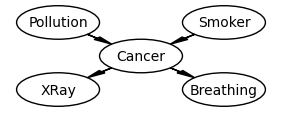
\includegraphics[scale=0.6]{imgs/example_dag.png}
		\caption*{An example of Directed Acyclic Graph (DAG) \footnotemark}
	\end{figure}
	\begin{center}

	Each variable is conditionally independent of all non-descendants given its parents.

			$$ \text{\emph{XRay}} \ci \text{\emph{Pollution}} | \text{\emph{Cancer}} $$
			$$ \text{\emph{Breathing}} \ci \text{\emph{Smoker}} | \text{\emph{Cancer}} $$
	\end{center}
	\footnotetext[1]{\footnotesize{K. B. Korb, A. E. Nicholson. Bayesian Artificial Intelligence}}
\end{frame}

\begin{frame}[fragile]
	\frametitle{Motivation: Model Testing}
	\begin{itemize}
		\setlength\itemsep{1em}
		\item In applied research, most of the DAGs are made by hand
			based on domain knowledge.
		\item Important to test whether the model is consistent with the data.
		\item Conditional Independence (CI) tests can be used to verify model structure.
	\end{itemize}
	\begin{figure}
 	\begin{verbatim}
	                              x2 df    p.value
	 Brth _||_ Pllt | Cncr 4.7571803  2 0.09268115
	 Brth _||_ Smkr | Cncr 9.0058063  2 0.01107679
	 Brth _||_ XRay | Cncr 1.9104270  2 0.38472999
 	\end{verbatim}
		\caption*{Example model testing output from R package \emph{dagitty}}
	\end{figure}

\end{frame}

\begin{frame}
	\frametitle{Motivation: Structure Learning}
	\begin{itemize}
		\setlength\itemsep{1em}
		\item CI implies that no direct causal link exists between the variables. \newline
			$ \text{\emph{XRay}} \ci \text{\emph{Smoker}} | \text{\emph{Cancer}} \implies \text{No edge b/w \emph{XRay} and \emph{Smoker}} $

		\item Constraint-Based structure learning algorithms like PC
			and FCI use CI tests to systematically search for CIs
			in the dataset to determine model skeletons.
	\end{itemize}
	\begin{figure}
		\centering
		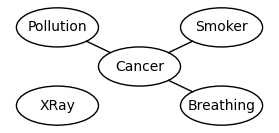
\includegraphics[scale=0.6]{imgs/example_sl.png}
		\caption*{Structure Learning Example}
	\end{figure}
\end{frame}

\section{Background}
\begin{frame}
	\frametitle{(Conditional) Independence}
	\begin{block}{Independence}
		Two random variables $ X $ and $ Y $ are independent,
		$ X \ci Y $ if and only if $ P(X, Y) = P(X) \cdot P(Y) $.
	\end{block}
	\vspace{1em}

	\begin{block}{Conditional Independence}
		Two random variables $ X $ and $ Y $ and are said to be
		conditionally independent given $ \bm{Z} $, $ X \ci Y | \bm{Z}
		$ if and only if for all $ z $ with $ p(z) > 0 $, $ P(X, Y |
		Z=z) = P(X | Z=z) \cdot P(Y | Z=z) $
	\end{block}
\end{frame}

\begin{frame}
	\frametitle{CI Testing is Difficult}
	\begin{figure}
		\centering

		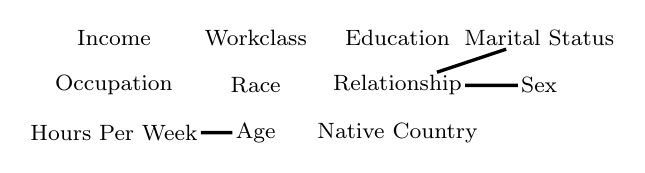
\begin{tikzpicture}[scale=0.6]
		\tikzstyle{every node}=[align=center, inner sep=1pt]
		\node at (0,0) {\footnotesize Income};
		\node at (3,0) {\footnotesize Workclass};
		\node at (6,0) {\footnotesize Education};
		\node (mrts) at (9 ,0) {\footnotesize Marital~Status};
		
		\node at (0,-1) {\footnotesize Occupation};
		\node (rltn) at (6,-1) {\footnotesize Relationship};
		\node at (3,-1) {\footnotesize Race};
		\node (sex) at (9,-1) {\footnotesize Sex};
		
		\node (hrpw) at (0,-2) {\footnotesize Hours~Per~Week};
		\node at (6,-2) {\footnotesize Native~Country};
		\node (age) at (3,-2) {\footnotesize Age};
		\draw [very thick] (sex) -- (rltn);
		\draw [very thick] (mrts) -- (rltn);
		\draw [very thick] (hrpw) -- (age);
		\end{tikzpicture}
		\caption*{Learned structure for US census income dataset using chi-square test}
	\end{figure}
	\begin{itemize}
		\item Testing for CI is much harder compared to testing for
			non-conditional independence.
		\item Especially in case of high cardinality or high number of
			conditional variables.
		\item In the continuous case, no test can exist which is calibrated and
			has power over all distributions where CI is True. \footnotemark
		\item Many different approaches and tests have been proposed.
	\end{itemize}

	\footnotetext[2]{\footnotesize{Shah, Rajen D., and Jonas Peters. "The hardness of conditional independence testing and the generalised covariance measure." The Annals of Statistics, 2020}}
\end{frame}

\begin{frame}
	\frametitle{Main classes of tests}
	\begin{itemize}
		\setlength\itemsep{1em}
		\item Stratification based tests
		\item Variable Importance based tests
		\item Residulaization based tests
	\end{itemize}
\end{frame}

\begin{frame}
	\frametitle{Stratification Based Tests}
	\begin{itemize}
		\setlength\itemsep{1em}
		\item Most common type for discrete variables. E.g. chi-square, G-test,
			mutual information based test, etc. 
		\item Converts CI test into simple independence test by splitting 
			the dataset.
		$ D[X, Y, \bm{Z}] = \{ D[X, Y, \bm{Z}=\bm{z_1}], D[X, Y, \bm{Z}=\bm{z_2}], \cdots \} $	
		\item Runs test on each stratum and then combines the results.
	\end{itemize}
\end{frame}

\begin{frame}
	\frametitle{Statification Based Test Example: Chi-squared}
	\begin{block}{}
	\begin{columns}
		\begin{column}{0.25 \textwidth}
			\begin{block}{\centering D}
			\begin{tabular}{c c c}
				X  & Y  & Z \\
				\hline
				X1 & Y1 & Z1 \\
				X1 & Y2 & Z2 \\
				X2 & Y1 & Z1 \\
				X3 & Y3 & Z2 \\
				\vdots & \vdots & \vdots \\
			\end{tabular}
			\end{block}
		\end{column}
		\begin{column}{0.25 \textwidth}
			\begin{block}{\centering $D_1$}
				\begin{tabular}{c c c}
					X & Y & Z \\
					\hline
					X1 & Y1 & Z1 \\
					X2 & Y1 & Z1 \\
					\vdots & \vdots & \vdots \\
				\end{tabular}
			\end{block}
			\begin{block}{\centering $ D_2 $}
				\begin{tabular}{c c c}
					X & Y & Z \\
					\hline
					X1 & Y2 & Z2 \\
					X3 & Y3 & Z2 \\
					\vdots & \vdots & \vdots \\
				\end{tabular}
			\end{block}
			\begin{block}{\centering $ D_i $}
			\end{block}
		\end{column}
		\begin{column}{0.5 \textwidth}
			\begin{block}{}
				$(X \ci Y)_{D_1} \to \chi_{D_1} $ and $ df_{D_1} $.
			\end{block}
			\begin{block}{}
				$(X \ci Y)_{D_2} \to \chi_{D_2} $ and $ df_{D_2} $.
			\end{block}
			\begin{block}{}
				$(X \ci Y)_{D_i} \to \chi_{D_i} $ and $ df_{D_i} $.
			\end{block}
		\end{column}
	\end{columns}
	\end{block}
	\begin{block}{}
		\centering
		$ (X \ci Y | Z)_{D} \to \sum_i \chi_{D_i} $ and $ df_{D} = \sum_i df_{D_i} $
	\end{block}
\end{frame}

\begin{frame}
	\frametitle{Stratification Based Tests: Advantages/Disadvantages}
	\begin{itemize}
		\item As the number of conditional variables is increased, exponentially
			less data is available in each stratum.
		\item Looses power when number of conditonal variables
			are increased.
	\end{itemize}
\end{frame}

\begin{frame}
	\frametitle{Variable Importance Tests}
	\begin{itemize}
		\setlength\itemsep{1em}
		\item Based on comparing the probability models: $\hat{p}(x |
			y, z) $ and $ \hat{p}(x | z) $. E.g. Stochastic
			Complexity-Based Conditional Independence Test (SCCI) \footnotemark.
		\item If the simpler model doesn't fit significantly worse, implies $ X \ci Y | Z $.
	\end{itemize}
	\footnotetext[3]{\footnotesize Marx, Alexander, and Jilles Vreeken. "Testing conditional independence on discrete data using stochastic complexity." PMLR, 2019}

\end{frame}

\begin{frame}
	\frametitle{Variable Importance Test Example: SCCI}
\end{frame}

\begin{frame}
	\frametitle{Variable Importance Tests: Advantages/Disadvantages}
	\begin{itemize}
		\item Can utilize any statistical model for which a reasonable goodness
			of fit exist.
		\item Inherently asymmetrical. The result of $ X \ci Y | Z $
			can be different from $ Y \ci X | Z $.
	\end{itemize}

\end{frame}

\begin{frame}
	\frametitle{Residualization Based Tests}
	\begin{itemize}
		\setlength\itemsep{1em}
		\item Uses two estimators $ \mathbb{E}[X| Z] $ and $
			\mathbb{E}[Y | Z] $ and checks for the multiplicative
			association between the residuals. E.g.
			Partial Correlation test, generalized covariance measure etc.
		\item Relies on the theorem from Daudin [1980] \footnotemark 
			that under CI, if the estimators have ``valid'' residuals
			such that $ \mathbb{E}[R_{X|Z}] = \mathbb{E}[R_{Y|Z}] = 0 $,
			then $ \mathbb{E}[R_{X|Z} R_{Y|Z}] = 0 $.
	\end{itemize}
	\footnotetext[4]{\footnotesize Daudin, J. J. "Partial association measures and an application to qualitative regression." Biometrika, 1980}
\end{frame}

\begin{frame}
	\frametitle{Residualization Based Test Example: Partial-correlation}
	\begin{itemize}
		\item Train two linear regression models
			$$ E_1 = X \sim Z \; \; \; \; \; \; \; E_2 = Y \sim Z $$
		\item Predict $ X $ and $ Y $ using the estimators 
			$$ \hat{X} = E_1(Z) \; \; \; \; \; \; \; \hat{Y} = E_2(Z) $$
		\item Compute the residuals
			$$ R_X = X - \hat{X} \; \; \; \; \; \; \; R_Y = Y - \hat{Y} $$
		\item Use Pearson correlation test on $ R_X $ and $ R_Y $.
	\end{itemize}
\end{frame}

\begin{frame}
	\frametitle{Residualization Based Tests: Advantages/Disadvantages}
	\begin{itemize}
		\item Any estimator can be used as long as it has ``valid'' residuals.
		\item No easy way to define residuals for ordinal and categorical variables.
		\item No residualization based test exists for categorical or ordinal variables.
	\end{itemize}
\end{frame}

\section{Unified test for ordinal and categorical data}
\begin{frame}
	\frametitle{Unified test for all data types}
	\begin{itemize}
		\setlength\itemsep{1em}
		\item Residualization based approach.
		\item Uses Li-Shepherd (LS) residuals \footnotemark.
		\item Any unbiased estimator can be used.
		\item Empirical results shown using Logistic Regression (GLM) and Random Forest (RFT).
	\end{itemize}
	\footnotetext[5]{\footnotesize C. Li and B. E. Shepherd. "A new residual for ordinal outcomes." Biometrika, 2012}
\end{frame}


\begin{frame}
	\frametitle{Residual for oridnal variables: LS-Residuals}
	Given an ordinal variable $ Y $ and an estimate $ \hat{p}(y) $ of $
	p(y) $, LS-Residual for sample $ y_i $ is defined as:
	$$ R_{y_i} = \hat{p}(Y < y_i) - \hat{p}(Y > y_i) $$
	\vspace{1em}

	For the binary case with $ Y \in \{0, 1\} $:
	$$ R_{y_i} = y_i - \hat{p}(Y = 1) $$
	\vspace{1em}

	For the conditional case for sample $ (y|z)_i $,
	$$ R_{y_i | z_i} = \hat{p}(Y < y_i | Z=z_i) - \hat{p}(Y>y_i|Z=z_i) $$

\end{frame}

\begin{frame}
	\frametitle{Residual for ordinal variables: LS-Residuals Example}
	\begin{block}{Ordinal Variable}
		\vspace{1em}
			$ \hat{p}(y) = \begin{array}{llll} Y_0 & Y_1 & Y_2 & Y_3 \\ 0.1 & 0.3 & 0.5 & 0.1 \end{array} $
		\begin{itemize}
			\item If $ y = Y_2 $, $ R_{y} = \hat{p}(Y < Y_2) - \hat{p}(Y > Y_2) = 0.3 $
			\item If $ y = Y_3 $, $ R_{y} = \hat{p}(Y < Y_3) - \hat{p}(Y > Y_3) = 0.9 $
		\end{itemize}
	\end{block}
	\begin{block}{Binary Variable}
		$\hat{p}(Y) = \begin{array}{ll} Y_0 & Y_1 \\ 0.3 & 0.7 \end{array} $
		\begin{itemize}	
			\item If $ y = Y_0 $, $ R_{y} = Y_0 - \hat{p}(Y=1) = -0.7 $
			\item If $ y = Y_1 $, $ R_{y} = Y_1 - \hat{p}(Y=1) = 0.3 $
		\end{itemize}
	\end{block}
\end{frame}

\begin{frame}
	\frametitle{Residual for categorical variables: Using dummy encoding}
	\begin{block}{Dummy Encoding}
		Given a random variable, $ Y $ with $ 4 $ possible states: $ \{Y_0, Y_1, Y_2, Y_3 \} $
		\begin{equation*}
			\bm{y} = \left[ \begin{array}{c} Y_3 \\ Y_1 \\ Y_2 \\ \vdots \end{array} \right] = \left[ \begin{array}{cccc} 0 & 0 & 0 & 1 \\ 0 & 1 & 0 & 0 \\ 0 & 0 & 1 & 0 \\ \vdots & \vdots & \vdots & \vdots \end{array} \right]
		\end{equation*}
	\end{block}

	\begin{block}{Residual Example}
	$\hat{p}(Y) = \begin{array}{cccc} Y_0 & Y_1 & Y_2 & Y_3 \\ 0.1 & 0.3 & 0.5 & 0.1 \end{array} $
	\begin{itemize}
		\item If $ y = Y_2 $, $ \begin{array}{cccc} 0 & 0 & 1 & 0 \\ -0.1 & -0.3 & 0.5 & -0.1 \end{array} $
		\item If $ y = Y_1 $, $ \begin{array}{cccc} 0 & 1 & 0 & 0 \\ -0.1 & 0.7 & -0.5 & -0.1 \end{array} $
	\end{itemize}
	\end{block}	
\end{frame}

\begin{frame}
	\frametitle{Test Statistic: Both continuous or ordinal variables}
	$$ Q_1(\bm{x}, \bm{y}) = \frac{1}{n} \frac{(R_{\bm{x}} \cdot R_{\bm{y}})^2}{\bm{var}(R_{\bm{x}} R_{\bm{y}})} $$
	\begin{center}
		\begin{itemize}
			\item If $ X \ci Y | Z $, asymptotically $ Q_1(\bm{x}, \bm{y}) \sim \chi^2(1) $.
			\item $ R_{\bm{x}} $ and $ R_{\bm{y}} $ are vectors of residuals.
		\end{itemize}
	\end{center}
\end{frame}

\begin{frame}
	\frametitle{Test Statistic: One categorical and one ordinal}
	$$ Q_2(\bm{x}, \bm{y}) = \frac{1}{n} (d \times \hat{\Sigma}_d^{-1} \times d^T) $$

	\begin{equation*}
		\begin{split}
		d &= (R_{\mathbb{I}(\mathbf{x}=1)} \cdot R_{\mathbf{y}}, \, \ldots \ , R_{\mathbb{I}(\mathbf{x}=k-1)} \cdot R_{\mathbf{y}}) \\ 
		\hat{\Sigma}_d &= Cov([R_\mathbb{I}(\mathbf{x}=1) \odot R_\mathbf{y}, \cdots, R_\mathbb{I}(\mathbf{x}=k-1) \odot R_\mathbf{y}])
		\end{split}
	\end{equation*}
	\begin{center}
		\begin{itemize}
			\item If $ X \ci Y | Z $, asymptotically $ Q_2(\bm{x}, \bm{y}) \sim \chi^2(k-1) $.
			\item $ R_{\bm{x}} $ is a matrix of residuals with each column corresponding to a dummy state and $ R_{\bm{y}} $ is still a vector.
			\item One of the columns of the dummy encoded variable
				is dropped as it will be colinear. Including it will
				result in a non full-rank covariance matrix.
		\end{itemize}
	\end{center}
\end{frame}

\begin{frame}
	\frametitle{Test Statistic: Both categorical}

	$$ Q_3(\bm{x}, \bm{y}) = \frac{1}{n} (d \times \hat{\Sigma}_d^{-1} \times d^T) $$

	\begin{equation*}
		\begin{split}
		d = (&R_{\mathbb{I}(\mathbf{x}=1)} \cdot R_{\mathbb{I}(\mathbf{y}=1)}, \, \ldots \ ,
				R_{\mathbb{I}(\mathbf{x}=k-1)} R_{\mathbb{I}(\mathbf{y}=1)}, \, \ldots \, , \\
		     &R_{\mathbb{I}(\mathbf{x}=1)} \cdot R_{\mathbb{I}(\mathbf{y}=r-1)}, \, \ldots \ ,
				R_{\mathbb{I}(\mathbf{x}=k-1)} R_{\mathbb{I}(\mathbf{y}=r-1)}) 
		\end{split}
	\end{equation*}
	\begin{equation*}
		\hat{\Sigma}_d = Cov([R_\mathbb{I}(\mathbf{x}=1) \odot R_\mathbb{I}(\mathbf{y}=1), \cdots, R_\mathbb{I}(\mathbf{x}=k-1) \odot R_\mathbb{I}(\mathbf{y}=r-1)])
	\end{equation*}

	\begin{center}
		\begin{itemize}
			\item If $ X \ci Y | Z $, asymptotically $ Q_3(\bm{x}, \bm{y}) \sim \chi^2((k-1)(r-1)) $.
			\item Both $ R_{\bm{x}} $ and $ R_{\bm{y}} $ are matrices of residuals.
		\end{itemize}
	\end{center}

\end{frame}

\begin{frame}
	\frametitle{Test Summary}
	\begin{enumerate}
		\setlength\itemsep{1em}
		\item If $\mathbf{Z} = \emptyset $ , do a non-conditional chi-squared test.
		\item If either $ X $ or $ Y $ are non-binary categorical,
			dummy/one-hot encode them.
		\item Train two estimators $ E_x = \bm{x} \sim \bm{z} $ and
			$ E_y = \bm{y} \sim \bm{z} $
		\item Make probability predictions using these two estimators 
			$ \hat{p}(x) = E_x(\bm{z}) $ and $ \hat{p}(y) =
			E_y(\bm{\bm{z}}) $.
		\item Use predictions and true values to compute LS-Residuals $ R_{\bm{x}|\bm{z}} $ and $ R_{\bm{y}|\bm{z}} $.	
		\item Compute the test statistic and df.
	\end{enumerate}
\end{frame}

\begin{frame}
	\frametitle{Code Example}
	\todo[inline]{Show a code example of how it works}
\end{frame}

\begin{frame}
	\frametitle{Proof: M-estimation theory}
	\justifying{Given a vector of parameters $ \bm{\theta} $, and a function $ \Psi_i(\bm{\theta}) = \Psi(Y_i, X_i, \bm{Z}_i; \bm{\theta}) $, such that the following conditions are satisfied.}
	\begin{enumerate}
		\item $ \bm{\theta} $ can be estimated using $ \sum_{i=1}^n \Psi_i(\bm{\theta}) = 0 $.
		\item $ \Psi_i $ doesn't depend on $ i $ or $ n $.
		\item $ \mathbb{E}[\Psi_i(\bm{\theta})] = 0 $
	\end{enumerate}

	From m-estimation theory, if $ \Psi $ is suitably smooth, then as $ n \to \infty $,

	$$ \sqrt{n}(\hat{\bm{\theta}} - \bm{\theta}) \to \mathcal{N}(0, V(\bm{\theta})) $$
	where 
	\begin{equation*}
		\begin{split}
			V(\bm{\theta}) &= A(\bm{\theta}^{-1}) B(\bm{\theta})[A(\bm{\theta})^{-1}]' \\
			A(\bm{\theta}) &= \mathbb{E} \left[ - \frac{\partial}{\partial \bm{\theta}} \Psi_i(\bm{\theta}) \right] \\ 
			B(\bm{\theta}) &= \mathbb{E}[\Psi_i(\bm{\theta}) \Psi_i(\bm{\theta})]'
		\end{split}
	\end{equation*}

\end{frame}

\begin{frame}
	\frametitle{M-Estimator example: Linear Regression: ML Estimator}
	$$ Y = \bm{\beta} \bm{X} + \epsilon $$
	Log-likelihood function: $ l(X, Y; \bm{\beta}) = C - \frac{1}{2 \sigma^2} \sum_{i=1}^{N}(y_i - \bm{\beta} x_i)^2 $
	M-estimator = $ \frac{\partial}{\partial \bm{\beta}} l(X, Y; \bm{\beta}) $

	Implying $ \sqrt{n}(\hat{\bm{\beta}} - \bm{\beta}) = \mathcal{N}(0, V(\bm{\beta}) $.

\end{frame}

\begin{frame}
	\frametitle{M-Estimator and Delta method}
	\begin{block}{Delta Method}
		If there is a sequence of random variables $X_n$ satisfying $ \sqrt{n}[X_n - \theta] \rightarrow \mathcal{N}(0, \sigma^2) $, then
		$$ \sqrt{n}[g(X_n) - g(\theta)] \rightarrow \mathcal{N}(0, [g'(\theta)] \sigma^2 [g'(\theta)]')$$
	\end{block}
	\begin{block}{M-Estimator and Delta Method}
		Given a function $ g(\bm{\theta}) $ which is a smooth function of $ \bm{\theta} $, we have:

		$$ \sqrt{n} \left[ g(\hat{\bm{\theta}}) - g(\bm{\theta}) \right] \to \mathcal{N} \left( 0, \left[ \frac{\partial}{\partial \bm{\theta}} g(\bm{\theta}) \right] V(\bm{\theta}) \left[ \frac{\partial}{\partial \bm{\theta}} g(\bm{\theta}) \right]' \right) $$
	\end{block}
\end{frame}

\begin{frame}
	\frametitle{M-Estimator for the test statistic}
	\begin{itemize}
		\item Divide our parameter vector into $ 3 $ sets: $ \bm{\theta} = \{ \bm{\theta^\bm{X}}, \bm{\theta^\bm{Y}}, \bm{\theta^\bm{T}} \} $.
		\item $ \bm{\theta^\bm{X}} $ and $ \bm{\theta^\bm{Y}} $ stay the same for all test
			statistics:

			\begin{equation*}
			\Phi_i(\bm{\theta}) = \begin{cases}
				\frac{\partial}{\partial \bm{\theta}^{\bm{Y}}} l_Y (Y_i, \bm{Z}_i; \bm{\theta^{Y}}) \\
				\frac{\partial}{\partial \bm{\theta}^{\bm{X}}} l_X (X_i, \bm{Z}_i; \bm{\theta^{X}}) \\
				\end{cases}
			\end{equation*}

		\item $ l_X $ and $ l_Y $ are log-likelihood functions of the probability models $ P(X | \bm{Z}) $ and $ P(Y | \bm{Z}) $ with parameters $ \bm{\theta}^X $ and $ \bm{\theta}^Y $ respectively.
		\item We use this as a partial M-estimator for our test statistic and define $ \bm{\theta}^T $ for each of our test statistic.
	\end{itemize}
\end{frame}

\begin{frame}
	\frametitle{Proof: Both ordinal case}
	\begin{equation*}
		\begin{split}
			\bm{\theta}^T &= (\theta_1, \theta_2) \\
			\Psi (X_i, Y_i, \mathbf{Z}_i; \bm{\theta}^T) &= 
				\begin{cases}
					R_{y_i} R_{x_i} - \theta_1 \\
					(R_{y_i} R_{x_i})^2 - \theta_2
				\end{cases} \\
			g(\bm{\theta}) &= \frac{\theta_1}{\sqrt{\theta_2 - \theta_1^2}} \\
		\end{split}
	\end{equation*}


		% \begin{equation}
		% 	\begin{split}
		% 		\hat{\theta}_1 &= \mathbb{E}[R_{\mathbf{x}} R_{\mathbf{y}}] \\
		% 		\hat{\theta}_2 &= \mathbb{E}[(R_{\mathbf{x}} R_{\mathbf{y}})^2] \\
		% 	\end{split}
		% \end{equation}

	\begin{itemize}
		\item $ g(\bm{\theta}) $ is chosen such that $ Q_1 = (\sqrt{n} g(\bm{\theta}))^2 $.
		\item As $ n \rightarrow \infty $, $ \sqrt{n} (g(\hat{\bm{\theta}}) - g(\bm{\theta})) \rightarrow \mathcal{N}(0, \sigma^2) $.
		\item Using $ \Psi(X_i, Y_i, \bm{Z}_i; \bm{\theta}^T) = 0 $: 
			$$ \hat{\theta}_1 = \mathbb{E}[R_{\mathbf{y}} R_{\mathbf{x}}], \hat{\theta}_2 = \mathbb{E}[(R_{\mathbf{x}} R_{\mathbf{y}})^2] $$
		\item Since under the null $ g(\bm{\theta}) = 0 $, $\sqrt{n}g(\hat{\bm{\theta}}) \rightarrow \mathcal{N}(0, \sigma^2) $.
	\end{itemize}

\end{frame}

\begin{frame}
	\frametitle{Proof: One ordinal and one categorical case}
	\begin{equation*}
		\begin{split}
			& \bm{\theta}^T = (\bm{\theta_1}, \bm{\theta_2}) \\
			& \bm{\theta_1} = (\theta_1^1, \theta_1^2, \cdots, \theta_1^{k-1}) \\
			& \bm{\theta_2} = (\theta_2^{11}, \cdots, \theta_2^{1(k-1)}, \theta_2^{21}, \cdots, \theta_2^{2(k-1)}, \cdots, \theta_2^{(k-1) (k-1)}) \\
			& \Psi(X_i, Y_i, \mathbf{Z}_i; \bm{\theta}^T) = 
				\begin{cases}
					R_{{\mathbb{I}(x=j)}_i}.R_{y_i} - \theta_1^j \, \, \forall j \in \{ 1, \cdots, k-1 \} \\
					(R_{{\mathbb{I}(x=j)}_i}.R_{y_i} \times R_{{\mathbb{I}(x=k)}_i}.R_{y_i}) - \theta_{2}^{jk} \,\, \forall j, k \in \{ 1, \cdots, k-1 \} \\
				\end{cases} \\
			& g(\bm{\theta}) = \bm{\theta_1} \bm{\wedge}
		\end{split}
	\end{equation*}

	where:
\begin{equation*}
	\begin{split}
		\bm{\wedge} &= \bm{\Sigma}^{-\frac{1}{2}} \\
		\Sigma^{i,j} &= \mathbb{E}[(R_{\mathbb{I}(\mathbf{x}=i)}.R_\mathbf{y})(R_{\mathbb{I}(\mathbf{x}=j)}.R_\mathbf{y})] - \mathbb{E}[R_{\mathbb{I}(\mathbf{x}=i)}.R_\mathbf{y}] \mathbb{E}[R_{\mathbb{I}(\mathbf{x}=j)}.R_\mathbf{y}] \\
			    &= \theta_2^{ij} - \theta_1^{i} \theta_1^{j} \\
	\end{split}
\end{equation*} 
\end{frame}

\section{Test performance}
\begin{frame}
	\frametitle{Empirical Analysis: Calibration}
	\begin{itemize}
		\item Under the null (i.e. $ X \ci Y | Z $), the p-value should
			be uniformly distributed.
		\item We test the distribution of p-values on simulated
			datasets with varying sample sizes and number of
			conditional variables.
		\item Independent datasets are generated using the DAG:
			\begin{figure}
				\centering
				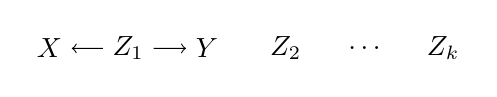
\begin{tikzpicture}[yscale=.75]
				\node (x) at (0,1) {$X$};
				\node (y) at (2,1) {$Y$};
				\node (z) at (1,1) {$Z_1$};
				\node at (3,1) {$Z_2$};
				\node at (4,1) {$\ldots$};
				\node at (5,1) {$Z_k$};
				\draw [->] (z) -- (y);
				\draw [->] (z) -- (x);
				\end{tikzpicture}
			\end{figure}
	\end{itemize}
\end{frame}

\begin{frame}
	\frametitle{Empirical Analysis: Calibration}
	\begin{figure}
		\centering
		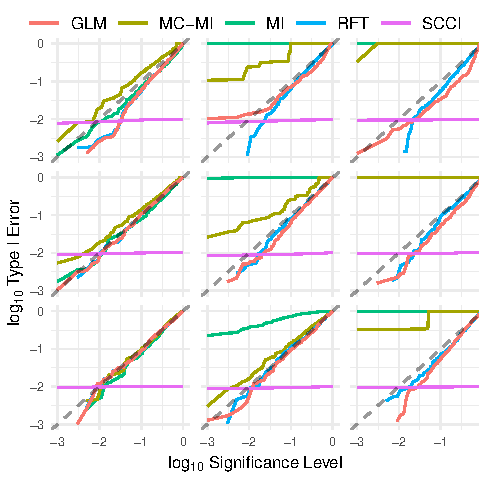
\includegraphics[scale=0.8]{imgs/calibration_add_vars.pdf}
		\caption*{Type I error vs significance level for sample sizes (top to
		bottom): $ [20, 40, 80] $ and number of conditional variables (left to
		right): $ [1, 3, 5] $ on conditionally independent simulated binary
		datasets.}
	\end{figure}
\end{frame}

\begin{frame}
	\frametitle{Empirical Analysis: Discrimination Data generation}
	\begin{itemize}
		\item When the null hypothesis is false, the test should be able to reject the null i.e. should have power.
		\item We test the accuracy of correctly classifying datasets as dependent or independent.
		\item Dependent datasets are generated with varying effect strength for $ X \to Y $. Additional independent conditional variables are added as noise.
			\begin{figure}
					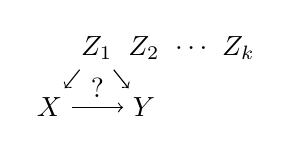
\begin{tikzpicture}[yscale=.75, xscale=.6]
						\node (x) at (0,0) {$X$};
						\node (y) at (2,0) {$Y$};
						\node (z) at (1,1) {$Z_1$};
						\node at (2,1) {$Z_2$};
						\node at (3,1) {$\ldots$};
						\node at (4,1) {$Z_k$};
						\draw [->] (x) edge node [midway, above] {?} (y);
						\draw [->] (z) -- (y);
						\draw [->] (z) -- (x);
					\end{tikzpicture}
			\end{figure}
		\item Independent datasets are generated by setting the effect to $ 0 $.
	\end{itemize}
\end{frame}

\begin{frame}
	\frametitle{Empirical Analysis: Discrimination}
	\begin{figure}
		\centering
		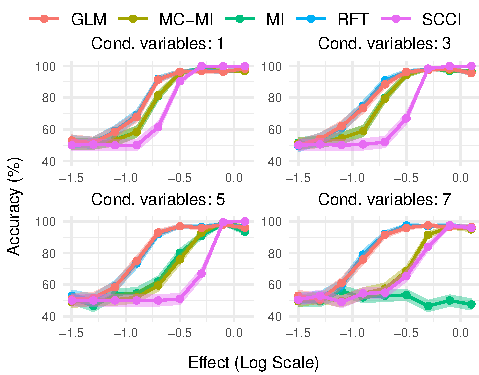
\includegraphics{imgs/accuracy.pdf}
		\caption*{Accuracy (shading: mean $\pm$ standard error, $N=200$)
		of classifying simulated binary datasets (sample size: $1000$)
		as conditionally dependent or independent.}
	\end{figure}

\end{frame}

\begin{frame}
	\frametitle{Epirical Analysis: Discrimination Data Generation (Ordinal)}
	Similar analysis as last one but for ordinal datasets.
\end{frame}

\begin{frame}
	\frametitle{Empirical Analysis: Discrimination (Ordinal)}
	\begin{figure}
		\centering
		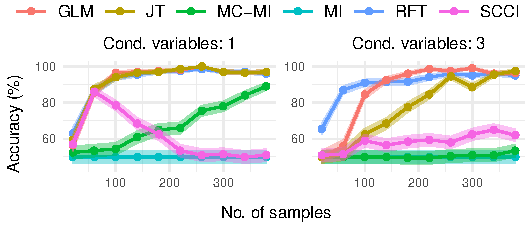
\includegraphics{imgs/accuracy_ordinal.pdf}
		\caption*{Accuracy (shading: mean $\pm$ standard error) of
		classifying simulated ordinal data (8 levels per variable) as
		conditionally dependent or independent.}	
	\end{figure}
	\footnotetext[7]{JT = Jonckheere-Terpstra test}
\end{frame}

\begin{frame}
	\frametitle{Applications: Model testing Data generation}
	\begin{itemize}
		\item Given a DAG and a dataset, how well is the test able to detect the implied CIs of the DAG in the data.
		\item We generate random DAGs with varying edge density 

			to generate implied CIs with varying number of conditional variables.
		\item Test the precision and recall of identify implied CI in the simulated dataset.
	\end{itemize}
\end{frame}

\begin{frame}
	\frametitle{Applications: Model testing}
	\begin{figure}
		\centering
		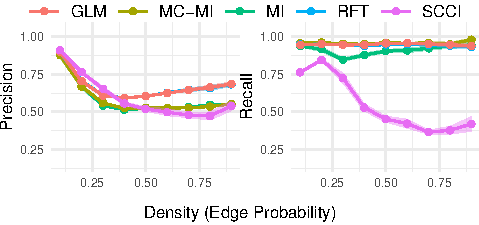
\includegraphics{imgs/model_testing.pdf}
		\caption*{Precision and recall (shading: mean $\pm$ standard
		error) of testing implied CIs and equal number of randomly
		generated CIs in binary datasets (sample size: $1000$)
		simulated from random DAGs on $ 20 $ variables.}
	\end{figure}
\end{frame}

\begin{frame}
	\frametitle{Constraint-Based Structure Learing}
	\begin{itemize}
		\item Systematically performs CI tests on a given dataset to construct a network structure.
		\item Starts with a fully connected network and removes edges $ X \to Y $ if $ X \ci Y | Z $ in data.
		\item The number of variables in $ Z $ is increased in each iteration.
		\item The algorithm reaches higher number of conditional variables in denser graphs.
	\end{itemize}
	\todo[inline]{Show an example}
\end{frame}

\begin{frame}
	\frametitle{Applications: Structure Learning data generation}
	\begin{itemize}
		\item Test how well is the test able to recover a DAG from given dataset.
		\item Generated random DAGs while varying the edge probability and simulated datasets from it.
		\item PC algorithm is used to learn the DAG back from the simulated datasets.
		\item We compare the edges in the learned and the original DAG.
	\end{itemize}
\end{frame}

\begin{frame}
	\frametitle{Applications: Structure Learning}
	\begin{figure}
		\centering
		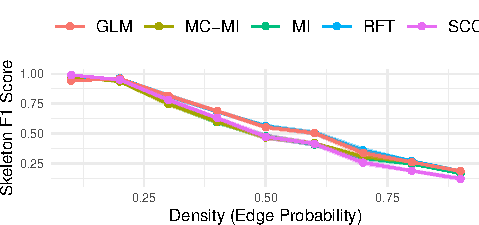
\includegraphics{imgs/sl_density.pdf}
		\caption*{Structure learning on simulated data. F1-score
		(shading: mean $\pm$ standard error) of the learned model
		skeletons for randomly generated DAGs with $20$ variables and
		varying edge probabilities.}
	\end{figure}
\end{frame}

\begin{frame}
	\frametitle{Applications: Structure Learning}
	\begin{figure}
		\centering
		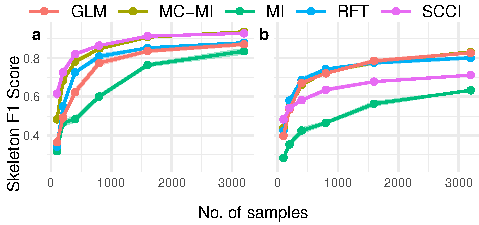
\includegraphics{imgs/sl.pdf}
		\caption*{Structure learning on (a) ``alarm'', and (b)
		``insurance'' datasets.  F1-score (shading: mean $\pm$ standard
		error, $N=10$) of the learned model skeletons.}
	\end{figure}
\end{frame}

\begin{frame}
	\frametitle{Applications: Structure Learning}
	\begin{figure}
		\centering
		\begin{subfigure}{0.5\textwidth}
			\centering
			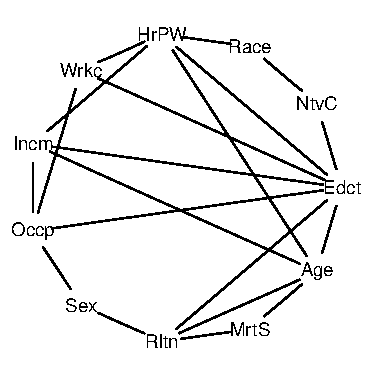
\includegraphics[scale=0.85]{imgs/sl-adult-rf.pdf}
			\caption*{}
			\label{fig:sl_adult_model}
		\end{subfigure}%
		\begin{subfigure}{0.5\textwidth}
			\centering
			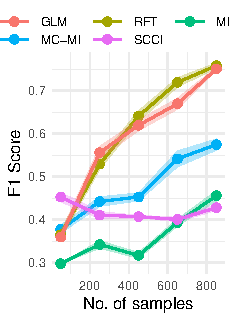
\includegraphics{imgs/adult_F1.pdf}
			\caption*{}
			\label{fig:sl_adult}
		\end{subfigure}
		\caption*{Structure learning on US census income dataset. (a)
		Learnt skeleton using RFT. (b) F1-score (shading: mean $\pm$
		standard error, $N=10$) when comparing $d$-connected variable
		pairs from the CPDAG to correlated variable pairs in the
		dataset.}
	\end{figure}
\end{frame}

\begin{frame}
	\frametitle{Runtime Analysis}
	\begin{figure}
		\centering
		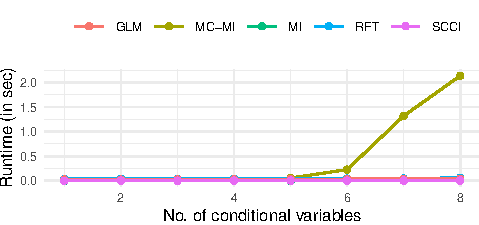
\includegraphics{imgs/runtime.pdf}
		\caption*{Runtime (shading: mean $\pm$ standard error, $N=100$)
		for CI tests with varying numbers of conditional variables and
		$1000$ samples per dataset.
		}
	\end{figure}
\end{frame}

\section{Conclusion}
\begin{frame}
	\frametitle{Conclusion/Future Work}
	\begin{itemize}
		\setlength\itemsep{1em}
		\item A residualization based CI test that works for a combination of ordinal and categorical variables.
		\item Properties: 1) Simple to implement; 2) Interpretable chi-square test statistic; 3) Symmetric by construction; 4) Computationally feasible
		\item Performs reasonably well for low number of
			conditional variable but performs better for high
			number of conditional variables.
		\item For structure learning, a hybrid approach can be used with other
			tests.
		\item Since Random Forests can work with combination of discrete and 
			continuous variables, can possibly be extended to a single 
			unified test.
	\end{itemize}
\end{frame}

\begin{frame}
	\begin{center}
		\Huge{Thanks for listening} \newline
		\Huge{Questions}
	\end{center}
	\begin{center}
		Paper preprint: https://arxiv.org/pdf/2206.04356.pdf
	\end{center}
\end{frame}

\end{document}
